\cotefile{157-4}
\scanpage{148}\mspage{22}
de cardinal majoré par
\[
\underset{\begin{gathered}\text{\unsure{nb de ces|nb des|nb de classes}}\\\text{syst. inductifs}\\\text{dans }\uuline{M}^{\pi},\ \unsure{?|\text{à}}\\\text{isom près}\end{gathered}}{
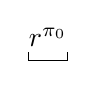
\begin{tikzpicture}[baseline=(a.base)]
\node[inner sep=0pt] (a) {$r^{\pi_0}$};
\draw ([yshift=-2pt]a.south west)--++(0,-3pt)-|([yshift=-2pt]a.south east);
\end{tikzpicture}}
\cdot
\underset{\begin{gathered}\text{\unsure{nb des|nb de}}\\\text{flèches d'un}\\\text{tel syst. ind.}\\\text{dans }X\end{gathered}}{
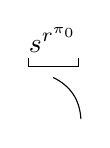
\begin{tikzpicture}[baseline=(b.base)]
\node[inner sep=0pt] (b) {$s^{r^{\pi_0}}$};
\draw ([yshift=-2pt]b.south west)--++(0,-3pt)-|([yshift=-2pt]b.south east);
\draw ([yshift=-9pt]b.south) to[bend left=30] ++(10pt,-15pt);
\end{tikzpicture}}
=s^{r^{\pi_0}}.
\]
Mais il faut maintenant faire varier $I$, à isom près, dans \unsure{la|le} cat des ens. ordonnés (\unsure{filtrants|filtrant} \unsure{etc|et}) de cardinal $\unsure{\le|\ge}\inserted{\lambda=}\unsure{r}^{\pi_0}\deleted{\unsure{\mathrm{card}\,I|\mathrm{card}}}$. On voit de suite que cet ensemble des classes d'isomorphie (qui peut s'interpréter comme un quotient d'\deleted{\unsure{l'|un}}\inserted{un certain} ens \unsure{de|des} \unsure{parties|relations} d'un ens. fixe $I_0$ de card $\lambda$) est de cardinal $\le2^\lambda$.
On trouve donc finalement
\[
\mathrm{card}\,\widetilde{M^r_{/X}}\le s^{(r^{\pi_0})}\cdot2^{(r^{\pi_0})}=s^{(r^{\pi_0})},
\]
sous condition que
\[
r\ge\mathrm{Sup}(\pi_1,C_0),\qquad s\ge\mathrm{Sup}(\pi_1,C_1).
\]
Il faut prouver l'inégalité similaire pour $\mathrm{card}\,\widetilde{\underline{\mathrm{Fl}}^r M}$ (3.9.). Or, \deleted{\unsure{le même calcul|le même cardinal|pour un cardinal}} pour \unsure{tt} $A,B$ dans $M^r$, on a si $r\ge\mathrm{Sup}(\pi_1,C_1)$
\[
\mathrm{card}\,\mathrm{Hom}_M(A,B)\le r^{(r^{\pi_0})}
\]
en vertu de (3.8) où on fait $s=r$, \unsure{on|et} \unsure{trouve|donc} que
\[
\begin{aligned}
\mathrm{card}\,
\underset{\deleted{\unsure{\mathrm{Fl}(M^r)|\mathrm{Fl}(M^r}\unsure{.}}}{
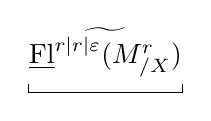
\begin{tikzpicture}[baseline=(c.base)]
\node[inner sep=0pt] (c) {$\widetilde{\underline{\mathrm{Fl}}^{\unsure{\deleted{r}|r|\varepsilon}}(M^r_{/X})}$};
\draw ([yshift=-2pt]c.south west)--++(0,-3pt)-|([yshift=-2pt]c.south east);
\end{tikzpicture}}
&\le\left(\mathrm{card}\,\widetilde{\unsure{M_{r/X}|M^r_{/X}}}\right)^2\cdot r^{(r^{\pi_0})}\\
&\le s^{(r^{\pi_0})}\cdot r^{(r^{\pi_0})}=s^{r^{\pi_0}},\\
&\text{si }s\ge r.
\end{aligned}
\]
% slanted
\margin{cf \unsure{cont.|corr.|cor.} p. 23}
(On va \unsure{regarder} plus bas le cas $s\le r^{\unsure{*|+}}$). C'est bien la formule (3.9.)
% archive sheet number: 147
